% This is samplepaper.tex, a sample chapter demonstrating the
% LLNCS macro package for Springer Computer Science proceedings;
% Version 2.20 of 2017/10/04
%
\documentclass[runningheads]{llncs}

% Packages 
\usepackage{graphicx} % Add assets folder to path for images. 
\graphicspath{{assets/}}
\usepackage{amsmath,amssymb,float,url} % Hide red underlines for URLs. 
\usepackage[hidelinks]{hyperref} % Stack two figures on top of each other.
\usepackage{subcaption} % Make caption text font smaller.
\usepackage{caption}
\captionsetup[figure]{font=small,labelfont=small}
% Make table-caption gap larger (source: https://bit.ly/3zm0wRn)
\captionsetup[table]{skip=10pt}

% Used for displaying a sample figure. If possible, figure files should
% be included in EPS format.
%
% If you use the hyperref package, please uncomment the following line
% to display URLs in blue roman font according to Springer's eBook style:
% \renewcommand\UrlFont{\color{blue}\rmfamily}

\begin{document}
%
\title{Machine Learning for Fish Oil Anaylsis}
%
%\titlerunning{Abbreviated paper title}
% If the paper title is too long for the running head, you can set
% an abbreviated paper title here
%
% \author{Jesse Wood\inst{1}\orcidID{0000-0003-3756-2122} \and
%   Bach Hoai Nguyen\inst{1}\orcidID{1111-2222-3333-4444} \and
%   Bing Xue\inst{1}\orcidID{2222--3333-4444-5555} \and 
%   Mengjie Zhang\inst{1}\orcidID{2222--3333-4444-5555} \and 
%   Daniel Killeen\inst{2}\orcidID{2222--3333-4444-5555}
% }
% %
% \authorrunning{J. Wood, B. Nguyen, et al.}
% First names are abbreviated in the running head.
% If there are more than two authors, 'et al.' is used.
%
% \institute{Victoria University of Wellington, Te Herenge Waka, PO Box 600, Wellington 6140, New Zealand\\
%   \email{ \{jesse.wood, bach.nguyen, bing.xue, mengjie.zhang\}@ecs.vuw.ac.nz}\\
%   \and 
%   Plant and Food Research, Port Nelson, Nelson 7010, New Zealand\\
%   \email{daniel.killeen@plantandfood.co.nz}\\
% }

%
\maketitle              % typeset the header of the contribution
%
\begin{abstract}
  % The abstract should briefly summarize the contents of the paper in
  % 150--250 words.
  
  In fish processing worldwide, 60\% of fish is not served. 
  This fish wastage can be repurposed into other products such as fish oils and fish feed.
  It is difficult and requires domain expertise to effectively repurpose fish biomass.
  Gas chromatography (GC) can be used to identify tissue samples in fish processing.
  The existing analytical chemistry techniques for processing GC data are manual and time-consuming.
  To reduce biomass waste we must incentivise biomass re-use, we reduce this barrier of entry through automation. 
  Here, we explore classification algorithms for fish oil data that automate and significantly reduce the time required to process GC data.
  Visualisation is used to explore the interpretability of the models such that their efficacy can be verified for use in a factory setting.
  The fish oil data is high-dimensional and low sample size.
  
  \keywords{
    feature selection \and 
    classification \and
    gas chromatography \and 
    support vector machine \and 
    particle swarm optimization \and 
    high-dimensional data
  }
\end{abstract}

\section{Introduction}
\label{introduction}

% [x] - Discuss visualisation (interpretability) and the need for feature selection. 
% [ ] - Good my writing is easy to understand but may need to be more formal. 
% [ ] - Disconnect here, (1) to know the fish oil component, (2) to know the fish type/part, which comes first and why? 

Omega-3 supplements are a high-value product made by repurposing fish waste in food processing. 
The waste is further refined into fish oil capsules commonly bought and sold at pharmacies. 
Certain fish species and parts are richer in omega-3 fatty acids, this makes these samples high value. 
We can identify valuable fish oils by classifying their species and part.

Gas chromatography (GC) is a chemistry technique used to analyze fish oils \cite{eder1995gas}. 
It analyzes the chemical structure of a fish oil sample \cite{restek2018high}. 
The technique is used for quality assurance in food processing. 
To repurpose fish waste effectively we must know what is in it. 
Chemists manually compare GC samples to reference data to determine their class. 

Classification automates this process by training a model on an existing dataset manually labelled by chemists. 
Given a fish oil sample, we can identify the fish species (i.e. Bluecod, Tarakihi), and part (Head, Fin).
Many classifiers \cite{fix1989discriminatory,hand2001idiot,ho1995random,loh2011classification,cortes1995support} can used to indentify the class of an instance from its features. 
These models can be organized into five categories: instance-based, probabilistic, tree-based, bagging and kernel-based, respectively. 
In this paper, we evaluate the performance of each classifier on both datasets, then explore the representation for the best performing classifier \cite{kennedy1995particle} with visualization. 

Many feature selection methods \cite{liu1995chi2,ding2005minimum,kononenko1994estimating,kennedy1995particle} are available to eliminate redundant features. 
These methods can be grouped into four categories: statistics, information theory, similarity, and swarm intelligence, respectively. 
In this paper, the SVM classifier \cite{cortes1995support} is evaluated on the feature subsets selected by each FS method, on both datasets. 

By only using important features for classification, it is easier to interpret what features/patterns the SVM model utilises. 
Interpretable models are capable of troubleshooting and diagnosis by domain expertise in real-world applications.
A model that is both interpretable and accurate has the potential to be deployed in a factory setting, this eliminates the need for manual work.

\section{Background}
\label{background}

\subsection{Gas Chromatorgraphy}

% [x] - The figure is too small, 
% [x] - a figure not referenced in the text, needs to be referred to. 
% [ ] - clumsy GC re-work this description. 

Gas chromatography (GC) is a technique for the analysis of chemical compounds \cite{eder1995gas,restek2018high}.
The process separates compounds based on their boiling point and molecular weight.
A compound is injected as a liquid, then heat is applied to vaporize it into a gas. 
This process is referred to as a phase transition. 
The speed at which a compound is vaporized depends on its boiling point. 
The vaporized gases travel through a long coiled tube.
That tube has a detector at the end, this detects the rate and intensity at which compounds reach the tube's end. 

\begin{figure}[htb]
  \centering
  \caption{Gas Chromatograph from a Snapper's Skin}
  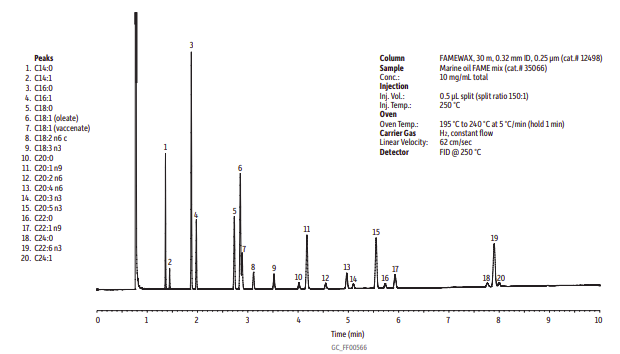
\includegraphics[width=12.5cm]{chromatograph.png}
  \label{fig:gas-chromatography} 
  \captionsetup[figure]{font=small,labelfont=small}
\end{figure}

Figure~\ref{fig:gas-chromatography} shows a gas chromatograph - the artefact of the GC method - from the dataset. 
This tissue sample was taken \emph{part} of skin, taken from the Snapper \emph{species}.
This chromatograph is the first instance of the fish oil dataset.
The detection is used to visualize intensity (y-axis) and time (x-axis) on a chromatograph. 
The distinguishable peaks are unique signatures where distinct chemical compounds can likely be identified.
Chemists match the peaks from known reference samples to classify unknown samples. 
Analysis can identify an unlabelled sample since they share similar peaks to previously labelled data.
There is noise in the peaks caused by time-shift - a known limitation of the measurement technique addressed in previous works \cite{tomasi2004correlation,zhang2008two}.

The existing task \cite{eder1995gas,restek2018high} of identifying compounds through chromatography is laborious.
Chemists integrate the area under each peak, and compare this to a reference sample, to classify the sample.
GC must be performed slowly to ensure that the peaks are not too broad.
This ensures each peak resolves and represents a single compound.
For this fish oil data, we classify a sample by two class labels - species and part. 
With intuition, fish from the same species share similar chemical compositions.
Machine learning techniques learn to recognize these patterns automatically, speeding up the process significantly. 
It can match a chromatograph to a target class, eliminating manual analysis. 

\subsection{Feature Selection}
\label{sec:background-feature-selection}

% goal -> efficient, interpretable models, simple models. 
% i.e. the m best features are not the best m features -> correlation and redundancy. 

There are two datasets with the same features. 
Those features are the high dimensional GC data, the class labels are the species and part.
The curse of dimensionality \cite{koppen2000curse} introduces problems: (1) computationally inefficient to evaluate the entire 4800 feature problem space. (2) Classification models are likely to overfit, learning noise in the data from irrelevant features. (3) Classifier models that utilize high-dimensional feature spaces are difficult to interpret, and it is difficult for domain experts to perform diagnoses or troubleshoot.

Figure~\ref{fig:gas-chromatography} shows at most several points of interest (peaks), and many negligible features, for an average chromatograph from the dataset. 

\begin{figure}[htb]
  \centering
  \caption{Feature Correlation Matrix}
  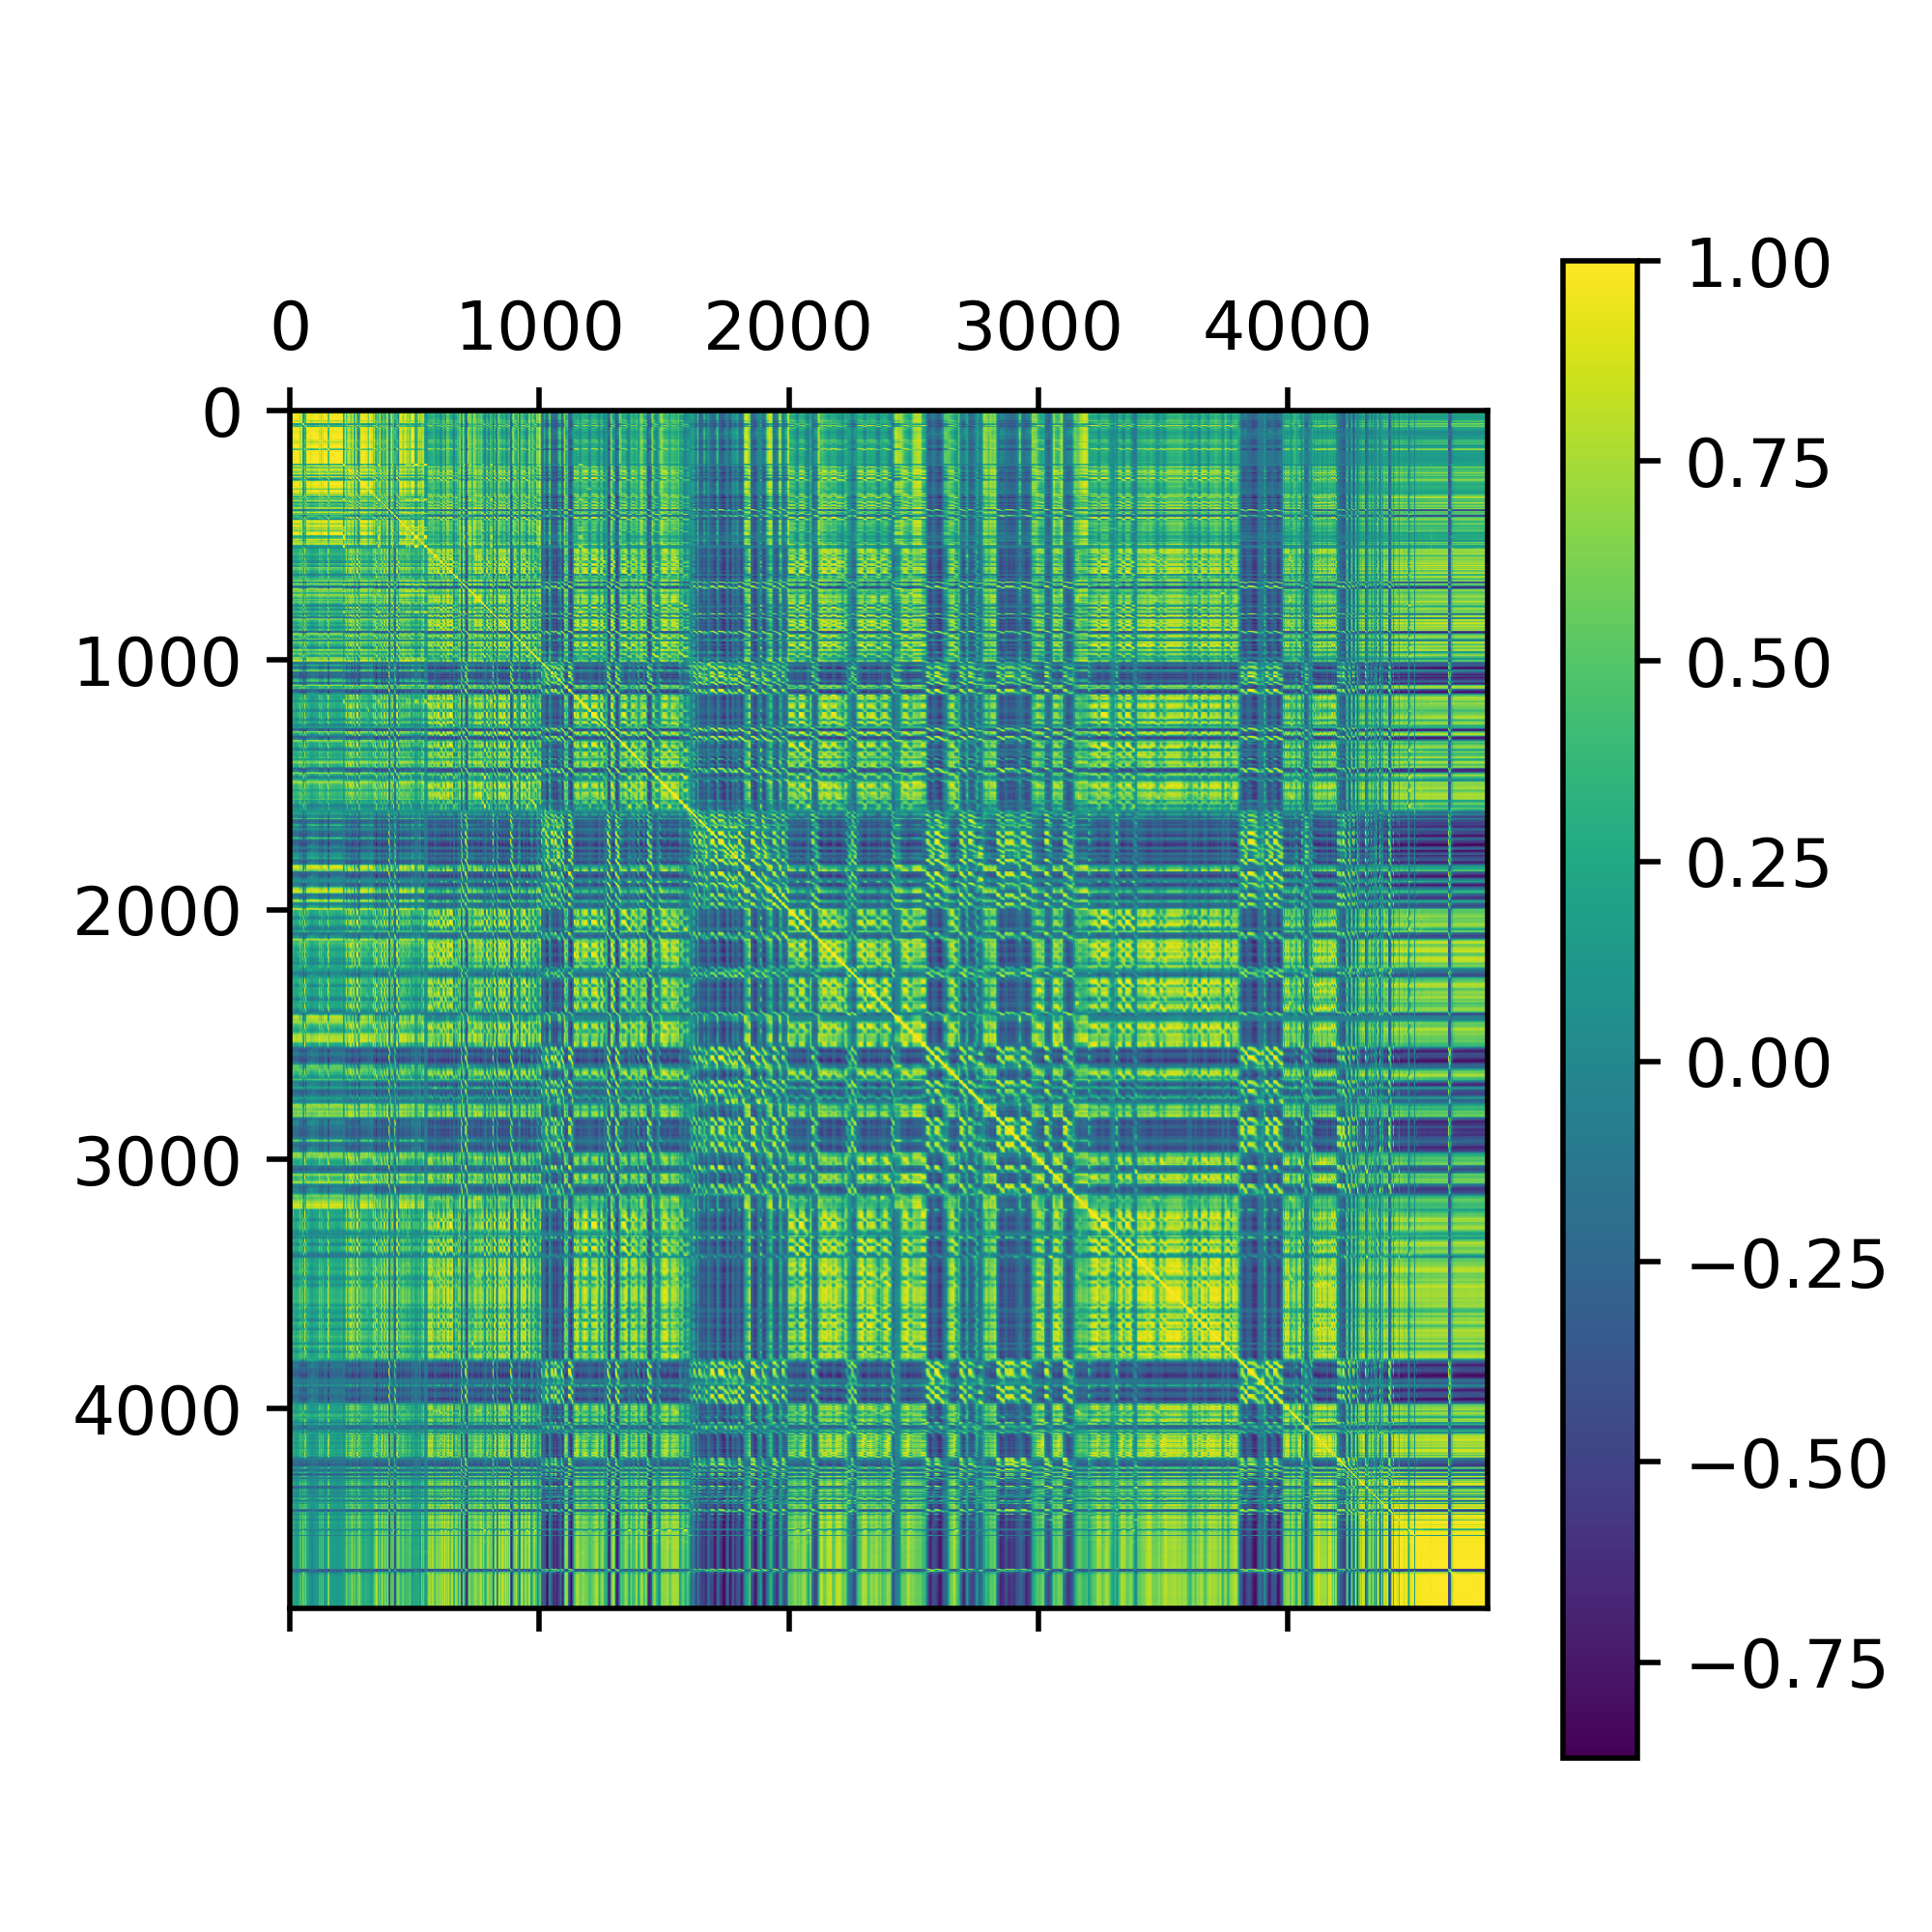
\includegraphics[width=8.5cm]{fish_correlation_matrix.png}
  \label{fig:correlation-matrix} 
  \captionsetup[figure]{font=small,labelfont=small}
\end{figure}

Figure~\ref{fig:correlation-matrix} gives the fish oil data pairwise correlation for the feature set using Pearson's correlation coefficient.
These figures illustrate the redundancy within the dataset, showing many irrelevant features. 
Feature selection reduces the size of the feature space by eliminating redundant and correlated attributes. 
To address these issues of high-dimensionality, we employ feature selection to select a subset of relevant features. 
Feature selection can (1) improve computational efficiency with a reduced dataset, (2) increase classification performance, and (3) lets classifiers produce simpler models which are in turn easier to troubleshoot.
We employ heuristic-based algorithms to address the combinatorial explosion of searching the possible feature subsets.
The algorithms used in this paper are introduced in further detail.

Liu et al. proposed Chi2 \cite{liu1995chi2}, a feature selection method via discretization. 
The algorithm is a generalized version of ChiMerge \cite{kerber1992chimerge} that determines a good $\chi^2$ threshold automatically from the data.

\begin{equation}
  \chi^2 = \sum_{i=1}^2 \sum_{j=1}^k \frac{(A_{ij} - E_{ij})^2}{E_{ij}}
  \label{eq:chi}
\end{equation}

The formula for calculating the $\chi^2$ statistic is given by eq.~(\ref{eq:chi}).
The technique performs both feature selection and discretization, making it ideal for continuous numeric fish oil data. 
The method can increase predictive performance, and efficiency (time/memory) and simplify models. 

Ding and Peng proposed Maximum-Redundancy Maximum-Relevance (MRMR) \cite{ding2005minimum} a feature selection method for gene microarray data. 
MRMR is a filter-based multi-objective method, 

\begin{equation}
  I(X;Y) = D_{KL}(P_{(X,Y)} || P_X \otimes P_X) 
  \label{eq:mutual-info}
\end{equation}  

These are both measured in terms of mutual information, given by eq.~(\ref{eq:mutual-info}), 
Let $(X,Y)$ be a pair of random variables, take the KL divergence \cite{kullback1951information} between their join distribution $P_{(X,Y)}$ and the product of their maginal distribution $P_X \otimes P_X$.

\begin{equation}
  f^{mRMR} = I(Y;X_i) - \frac{1}{|S|} \sum_{X_s \in S} I(X_s;X_i) 
  \label{eq:mrmr}
\end{equation}  

The MRMR feature importance score is given in eq.~(\ref{eq:mrmr}), for full derivation see \cite{liu1995chi2,zhao2019maximum}.
It balances both, the relevance for predicting outcome $I(Y;X_i)$, and the redundancy within features $I(X_s;X_i)$, scaled by the size of the feature subset $|S|$. 
It builds a set of features, adding the $X_i$ with the maximum feature importance to the selected subset.

Robnik proposed Relief-F \cite{kononenko1994estimating}, a feature selection method based on $k$ nearest neighbours. 
The algorithm extends Relief \cite{kira1992practical}, the extension is noise-tolerant, handles incomplete data and multi-class problems. 
Relief estimates feature importance based on their ability to separate other nearby instances.
With intuition, a good feature can distinguish between classes. 
Relief-F is noise tolerant by averaging the contribution of the $k$ nearest neighbours. 
Missing values of attributes are treated probabilistically\cite{robnik2003theoretical}.
Relief-F handles multi-class problems by taking the weighted average of near misses to all classes.

\begin{equation}
  W[A] := W[A] - \frac{1}{m} \left( diff(A,R,H) +  \sum_{C \ne class(R)} P(C) \times diff(A,R,M(C)) \right)
  \label{eq:reliefF}
\end{equation}

The attributes are estimated with the weight update function given by eq.~(\ref{eq:reliefF}). 

Kennedy and Eberhart proposed PSO \cite{kennedy1995particle} swarm intelligence method for non-linear optimization.
This imitates social behaviour, e.g. birds flocking or fish schooling.
Their synchronous movement was modelled as a function of each fish maintaining equal distance to its neighbours. 
To give intuition, we imagine a simple model of a schooling fish in search of food. 
With $p_{best}$ an individual fish's best spot, and $g_{best}$ the best spot the school has found. 
Each fish updates its movement in equal parts towards $p_{best}$ and $g_{best}$, both multiplied by a stochasticity factor.
The stochasticity introduces randomness, which makes the fish overshoot their target about half the time. 
The overshooting has fundamental to the success of the model, it allows the school to explore uncharted waters (unknown regions of the problem domain). 
% PSO walks the fine line between order (known local optima) and chaos (risky unknown regions).
The social model was simplified into a particle swarm, which allowed collisions where two particles share the same location. 

The fitness function used to determine $p_{best}$ and $g_best$, made suitable for feature selection, is given by

\begin{equation}
  fitness = C_1 * (1 - accuracy) + C_2 * k_{selected} / k_{total}  
  \label{eq:pso}
\end{equation}

Where $(1 - accuracy)$ is the error, $k_{selected} / k_{total}$ is the selection ratio.
$k_{selected}$ is the number of features chosen, and $k_{total} = 4800$ the size of the full feature set.
$C_1$ and $C_2$ are constants that scale the error and selection ratio, respectively.

\section{Data processing}

% TODO [ ] - Bach to fill out these sections. 

\begin{itemize}
  \item Why the raw data is not applicable to existing classification algorithms?
  \item Extracting datasets that are ready for classification algorithms:
        \begin{itemize}
          \item Sum up the intensity.
          \item Aligning missing packets.
        \end{itemize}
  \item Overview of extracted data.
\end{itemize}

\section{Classification}

% [x] 1. How do you perform classification here? 
% [x] 2. Splitting the data? 
% [x] 3. Training/test? 
% [x] 4. 10-fold cross-validation? 
% [x] 5. Why 30 independent runs? 
% [ ] - Provide a short description for each algorithm here! What are their parameter settings? 
% [ ] - Why KNN and NB have std != 0, these are deterministic methods. 
% [ ] - Overal steps 

In this section, we evaluate the performance of classifiers on the fish species and part dataset.
Classification identifies the class label of an instance from its features. 
An effective classifier has these desirable attributes: (1) high classification accuracy, (2) efficient computation, (3) and interpretable representation.
Classification accuracy should be equal to and/or greater than that of humans.
Any classifier that can perform the task in minutes rather than hours (how long it takes chemists manually) is preferred. 
An interpretable representation is required so troubleshooting and diagnoses can be performed by domain experts.
A classifier with these desirable attributes (1,2,3) can be utilized in a factory setting. 
\\\\
We compare 5 classifiers \cite{fix1989discriminatory,hand2001idiot,ho1995random,loh2011classification,cortes1995support} - k-Nearest Neighbours (KNN), Naive Bayes (NB), Random Forest (RF), Decision Trees (DT) and Support Vector Machines (SVM).
The average balanced classification accuracy by each classifier over 30 independent runs.
Central Limit Theorem says a sample distribution will approach a normal distribution $\mathcal{N}(\mu,\sigma)$, a sample size of 30 approximates a reliable measure of variance concerning the population. 
The datasets have a small sample size, so we use ten-fold cross-validation to create the training and test set.
K-fold stratification and balanced accuracy measures are used for each run. 
The balanced accuracy measure ensures results are not biased towards the mode class. 
In sum, this experiment gives 2 (datasets) x 5 (classifiers methods) x 30 (runs) = 300
sets of empirical performance results.

\subsection{Results and Discussion}

\begin{table}[htb]
  \captionsetup{font=small,labelfont=small}
  \caption{
    Classification Results
    }
  \centering
  \begin{tabular}{|l|l|l|l|l|}
    \hline
    Dataset                    & Method & 
    AvgTrain $\pm$ Std         & 
    % T                          &
    AveTest $\pm$ Std                      \\ % &
    % T                                     \\
    \hline
    Species                    & 
    \begin{tabular}[c]{@{}l@{}}
      KNN          \\ % K-Nearest Neighbors
      RF           \\ % Random Forest
      DT           \\ % Decision Tree
      NB           \\ % Naive Bayes
      \textbf{SVM} \\ % Support Vector Machine
    \end{tabular} & 
    \begin{tabular}[c]{@{}l@{}}
      83.57 $\pm$ 1.80         \\ % KNN
      100.00 $\pm$ 0.00          \\ % RF
      100.00 $\pm$ 0.00          \\ % DT
      79.54 $\pm$ 1.60         \\ % NB
      \textbf{100.00 $\pm$ 0.00} \\ % SVM
    \end{tabular} & 
    \begin{tabular}[c]{@{}l@{}}
      74.88 $\pm$ 12.54          \\ % KNN
      85.65 $\pm$ 10.76          \\ % RF
      76.98 $\pm$ 13.12          \\ % DT
      75.27 $\pm$ 4.35           \\ % NB
      \textbf{98.33 $\pm$ 5.00 } \\ % SVM
    \end{tabular}             \\
    \hline
    Part                       & 
    \begin{tabular}[c]{@{}l@{}}
      KNN          \\ % K-Nearest Neighbors
      RF           \\ % Random Forest
      DT           \\ % Decision Tree
      NB           \\ % Naive Bayes
      \textbf{SVM} \\ % Support Vector Machine
    \end{tabular} & 
    \begin{tabular}[c]{@{}l@{}}
      68.95 $\pm$ 3.49          \\ % KNN
      100.00 $\pm$ 0.00           \\ % RF
      100.00 $\pm$ 0.00           \\ % DT
      65.54 $\pm$ 2.69          \\ % NB
      \textbf{100.00 $\pm$ 0.00 } \\ % SVM
    \end{tabular} & 
    \begin{tabular}[c]{@{}l@{}}
      43.61 $\pm$ 13.48          \\ % KNN
      72.60 $\pm$ 16.15          \\ % RF
      60.14 $\pm$ 14.57          \\ % DT
      48.61 $\pm$ 12.19          \\ % NB
      \textbf{87.14 $\pm$ 8.52 } \\ % SVM
    \end{tabular}             \\
    \hline
  \end{tabular}
  \label{t:classification}
\end{table}

Table~\ref{t:classification} shows the results for KNN, RF, DT, NB, and SVM. 
It gives balanced classification accuracy with ten-fold cross-validation for each method. 
Results are given for fish species (top), and fish part (bottom) datasets. 
Results are averages across 30 independent runs for statistically significance. 
The mean and standard deviation of balanced accuracy is given using the fish species and part datasets. 
For each dataset, the best test accuracy is emphasized in bold. 

The SVM classifier outperforms the other classifiers on the test set, with 98.33\% and 87.14\% for species and part, respectively. 
It does so for the test set for both the species and part datasets.
For classifiers, KNN, DT and NB, for the species test it achieves 23.56\%, 21.35\%, 23.06\% better, and for the part test it achieves 12.26\%, 27\%, 38.53\% better, respectively.
NB assumes conditional independence between features.
Under this assumption, it cannot model complex relationships between dependent variables.
The chromatograph from figure~\ref{fig:gas-chromatography} shows a continuous and differentiable curve. 
The features at timestamps close to either side of a peak are also likely to be high. 
Conversely, features adjacent to a low intensity zero value are likely to also be low. 
The NB simply cannot model these feature interactions.

% More analysis needed here? 
% TODO [x] 1. Should compare algorithms performance based on number, e.g. SVM is 20% more accurate than KNN, DT, and NB. 
% TODO [x] 2. Why NB and KNN do not work well? 
% TODO [x] 3. Why DT overfit the data (you use full size)? 
% TODO [x] 4. RF is better because of the ensemble mechanism? 
% TODO [ ] 5. Too many features too few instances? 

The random forest, decision tree and support vector machine have perfect training accuracy.
The decision tree and random forest overfit the training data, achieving 100\% training accuracy on both datasets.
This accuracy is not reflected in the test data, where accuracy for both models is reduced, they cannot generalize to unseen data. 
By default, sklearn has no maximum depth for the decision tree.
Without a depth limit, the tree creates strict rules on sparse data and perfectly fits the training data.
It captures noise in the training set, that does not generalize to unseen data. 
Setting maximum depths or pruning redundant branches would address the overfitting. 

The RF classifier can generalize well, with SVM achieving, 12.68\% and 14.54\$ better than RF, on the fish species and part, respectively.
RF is 8.76\% and 12.46\% better than DT on the test set, for fish and species respectively. 
The ensemble mechanism makes RF more tolerant to noise than DT, it averages over many DT classifiers each operating on different subsets of the data. 
Also, the RF is noise-tolerant in comparison to KNN and NB.

The KNN struggles to notice the similarity in our n-dimensional where $n=4,800$, supported by train accuracy 83.57\% and 68.95\% for species and part, respectively. Tho model cannot fit the training data, let alone generalize effectively to the test, with 74.88\% and 43.61\% for species and part respectively. 
KNN struggles with high-dimensional data, as the number of dimensions increases the distance between similar instances also increases. 

\subsection{Discussion}
\label{sec:results-classification-discussion}

Classification accuracy for all models was better for the fish species than the part.
This suggests tissue samples for different species may have distinct chemical compositions.
Yet, different fish parts may have fewer underlying structural differences.
For GC data the intra-class variation between species provides a larger signal than part variation.
For example, we expect there to be more difference between a tarakihi and a bluecod, than there is a similarity between two livers from different species.

Of the techniques evaluated, the SVM outperformed the rest, providing the best test accuracy for both datasets. 
This model can identify fish species from gas chromatography data with near-perfect accuracy (98.33\%).
This model was a suitable candidate for automating the task, but can its reasoning be understood? 
This motivated further investigation into the representation of this technique.

\subsection{Weight Analysis}

% [x] - Replace 4.2 and 4.3 by weight analysis.
% [x] It is good that you perform different settings for SVM, 
% [x] but I doubt these additions would increase the paper's value. 
% [x] I remember you did analyse the weight vectors of the model to give an overview of some features may not be used. 
% [x] Such analysis is more valuable
% [x] - This part can be shortened, and, 
% [x] - included in the visualisation sections, (not background)
% [ ] Motivation for FS - It is also a good motivation for feature selection.

Model interpretability is explored through visualisation.
We aim to uncover learnt patterns that can be verified with domain knowledge.
The desired algorithm should strike a balance between predictive performance and semantically meaningful features.

What constitutes semantic meaning varies from one domain to another.
It is easy to build intuition for semantic meaning in computer vision and natural language processes, they correspond to recognisable images and structured text.
In the domains of gas chromatography and fish processing, our meaning is derived from performance on the classification task(s) and similarity to underlying chemical compounds.
We expect models that generate knowledge that can be verified with domain expertise. 
For example, important features will correspond to timestamps of important chemicals in the GC data.

\subsubsection{Support Vector Machines}

Cortes and Vapnik proposed the Support Vector Machine (SVM) \cite{cortes1995support}.
This model creates a hyperplane that can draw distinct class boundaries between classes.
We call these class boundaries the support vectors.
We are performing multi-class classification, so it used a one-vs-rest (OVR) approach \cite{sklearn2021feature}.
This creates a divide between one class and the rest, then repeats for the other classes.
The l1 regularization term leads to sparse models, these select fewer features. 
With fewer features, it becomes easier to interpret their meaning. 

SVM is generally considered a black box method. 
This is especially so with complex kernels such as radial base function (RBF), sigmoidal or polynomial. 
However, an analysis of a Linear kernel - as proven effective in our previous experiments - can provide meaningful interpretations. 
We explore the hyperplane coefficients to find important features for a given class. 

\subsubsection{Hyperplane}

The coefficients $\beta$ give you a vector in the n-dimensional ($n = 4800$) hyperplane.
Let $x$ be a vector for an instance in that same hyperplane.
The SVM model takes the dot product $\beta . x$ between the coefficients $\beta$ and instance $x$ to determine the class of $x$. 

\begin{equation}
  SVM  = \begin{cases} 
    \beta . x > 0 \quad Snapper \\
    \beta . x < 0 \quad Snapper \\
 \end{cases}
 \label{eq:svm}
\end{equation}

Equation~(\ref{eq:svm}) gives the piecewise function used to determine the positive class, in this example snapper. 
When $\beta . x$ is positive, the instance $x$ is classified as a snapper. 
Conversely, when $\beta . x$ is negative, the instance $x$ is not a snapper, and then the algorithm proceeds to the next hyperplane. 
Instances in training data will not lie directly on the hyperplane, i.e. $\beta . x = 0$, as it constructs an optimal hyperplane. 
The GC data, shown in figure~\ref{fig:gas-chromatography} is non-negative, all zero-valued or higher. 
This simplifies the dot product $\beta . x$ greatly, as only negative weights in $\beta$ can produce negative values.
The $\beta . x$ is the sum of element-wise product of $\beta$ and $x$. 
Positive weights push the sum towards the positive class a snapper. 
Negative weights push the sum towards the negative class, not a snapper. 

\subsubsection{Individual Hyperplane}

\begin{figure}[htb]
  \centering
  \caption[SVM Coef]{
      SVM Hyperplane Coeffecients
    }
  \begin{subfigure}[b]{.49\linewidth}
    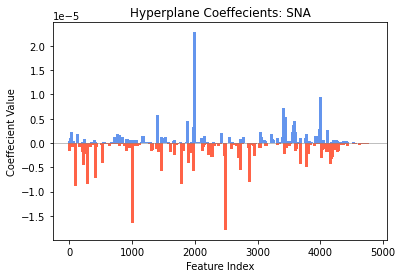
\includegraphics[width=\linewidth]{fish_hyperplane_sna.png}
    \caption{Snapper}\label{fig:hyperplane-sna}
  \end{subfigure}
  \begin{subfigure}[b]{.49\linewidth}
    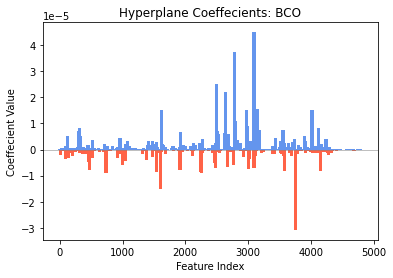
\includegraphics[width=\linewidth]{fish_hyperplane_bco.png}
    \caption{Bluecod}\label{fig:hyperplane-bco}
  \end{subfigure}
  \begin{subfigure}[b]{.49\linewidth}
    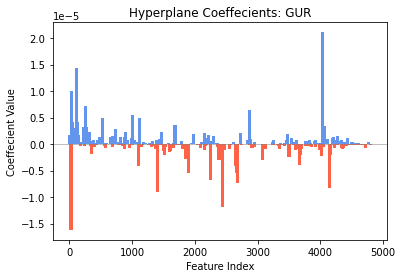
\includegraphics[width=\linewidth]{fish_hyperplane_gur.png}
    \caption{Gurnard}\label{fig:hyperplane-gur}
  \end{subfigure}
  \begin{subfigure}[b]{.49\linewidth}
    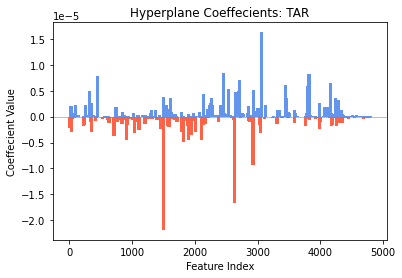
\includegraphics[width=\linewidth]{fish_hyperplane_tar.png}
    \caption{Tarakihi}\label{fig:hyperplane-tar}
  \end{subfigure}
  \label{fig:svm-hyperplane}
\end{figure}

Figure~\ref{fig:svm-hyperplane} shows the hyperplane coefficients for each class in the fish species dataset. 
The hyperplane coefficients are the weights assigned to each feature when drawing a support vector. 
We use colours to denote the sign of weight, a positive weight (blue), and a negative weight (red). 
Note, that the SVM uses OVR for multi-class problems, for classification each hyperplane is evaluated in sequential order.

\begin{figure}[htb]
  \centering  
  \caption[Two numerical solutions]{    
    Hyperplane coefficients $\beta_t$.
    }
  \begin{subfigure}[b]{.55\linewidth}
    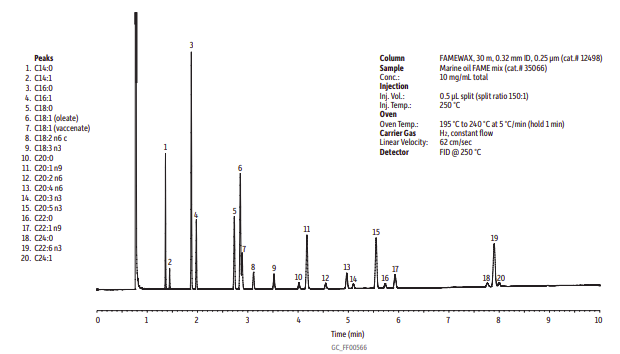
\includegraphics[width=\linewidth]{chromatograph.png}
    \caption{Species}\label{fig:fish-hyperplane-coeffcients}
  \end{subfigure}
  \begin{subfigure}[b]{.55\linewidth}
    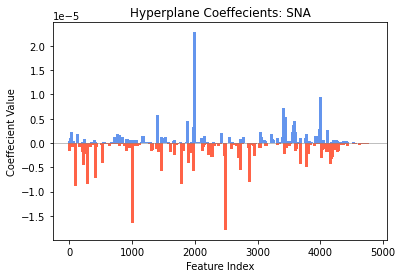
\includegraphics[width=\linewidth]{fish_hyperplane_sna.png}
    \caption{Part}\label{fig:part-hyperplane-coeffcients}
  \end{subfigure}
  \label{fig:hyperplane-chromatograph}
\end{figure} 

In figure~\ref{fig:hyperplane-chromatograph} we overlay a the snapper chromatograph $x$ (top) - previously from figure~\ref{fig:gas-chromatography}- with Snapper hyperplane coefficients $\beta$ (bottom).
From a cursory glance, low valued intensities $x$ correspond to the negative weights $\beta$.
Conversely, if they were peaks instead in $x$ would push the $\beta . x$ negative, away from the snapper class. 
In general, the higher value intensities $x$ including peaks, correspond to positive weights $\beta$. 
Peaks in $x$ for positive weights $\beta$, push $\beta . x$ positive, towards the positive class. 
Note that the largest peak, at timestamp $k = 653$, does not correspond to the largest weight $\beta$. 
This suggests, that while prominent for this instance, the feature at $k = 653$ on average does not have an important role in determining the snapper class. 
There are more large negative weights than positive, there are many important features that determine a class is not a snapper and fewer important weights that determine it is one. 

\subsubsection{Total Hyperplane}

Feature importance can be measured from the hyperplane coefficients. 
The absolute size of a coefficient relative to another gives a measure of its importance. 
Weights with large values have more impact on the position of the support vectors. 
To approximate the feature importance for an SVM, we can sum the absolute weights of the hyperplanes for each class, giving the \emph{total hyperplane}. 

\begin{align}\label{eq:hyperplane}
  \beta_{\text{t}} = \text{minmax}(
  \sum_{\text{c} \in \text{C}}
  |\beta_{\text{c}}|
  )
\end{align}

Equation~(ref{eq:hyperplane}) defines the total hyperplane.
Where $c$ is one class vs the rest hyperplane coefficient, and $C$ is the set of all classes. 
$\beta_{\text{t}}$ coefficient as the sum of hyperplane coefficients magnitude for each class $\beta_{\text{c}}$.
We normalize the coefficients with a min-max feature scaling.

\begin{figure}[htb]
  \centering  
  \caption[Two numerical solutions]{    
    Hyperplane coefficients $\beta_t$.
    }
  \begin{subfigure}[b]{.55\linewidth}
    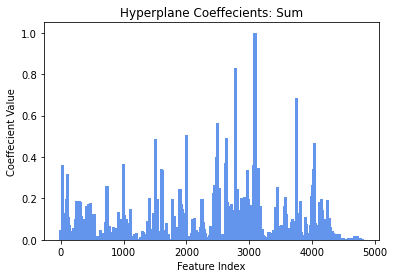
\includegraphics[width=\linewidth]{fish_total_coefficients.png}
    \caption{Species}\label{fig:fish-hyperplane-coeffcients}
  \end{subfigure}
  \begin{subfigure}[b]{.55\linewidth}
    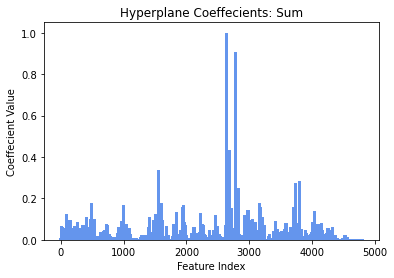
\includegraphics[width=\linewidth]{part_total_coefficients.png}
    \caption{Part}\label{fig:part-hyperplane-coeffcients}
  \end{subfigure}
  \label{fig:hyperplane-coefficients}
\end{figure} 

The total hyperplane for each dataset is given in Figure~\ref{fig:hyperplane-coefficients}.
The normalized sum of the magnitude of the coefficients for each class is given in Eq~\ref{eq:hyperplane}.
The absolute value operator removes the precision of the sign, we lose information about if a weight was positive or negative. 
This lost information makes the total hyperplane an approximation, not the full intuition behind the support vector machine. 
We can no longer reason on an individual class basis, as we did before. 
However, this approximation is still useful for reasoning with domain expertise. 
The outliers correspond to feature timestamps important for drawing class boundaries. 
These are chemical compounds that separate the fish part and species, respectively. 
We see many important features for fish species and far less for the fish part. 
The SVM model struggles to converge on a set of good features for the part dataset. 
This could explain why classification accuracy is worse for the fish part. 

\section{Feature Selection}

To find effective feature selection methods, we evaluate the classification performance of FS methods for a range of $k$ - where $k$ is the number of features selected - on the fish species and part dataset. Feature selection reduces the dimensionality of the problem space. FS methods identify and keep important features, and eliminate redundant ones. With fewer features contributing to the model's decisions, it becomes easier to troubleshoot and diagnose with domain expertise. By reducing the feature space we simplify the model, and simpler models become easier to understand. Feature selection can increases performance, both in terms of efficiency and accuracy. We can see if feature selection can improve the poor classification accuracy on the fish part dataset. 

As before with classification, we use ten-fold cross-validation to generate the training and test set. 
For each method, we measure balanced classification accuracy with an SVM model from \cite{sklearn2021feature}.
It has linear kernel, l1 regularization \cite{robnik2003theoretical} and 10,000 maximum iterations.
We use 3 feature selection methods \cite{liu1995chi2,ding2005minimum,kononenko1994estimating} - Chi2, MRMR, Relief-F - with implementation from \cite{li2018feature} set to their default parameters.
We use PSO from \cite{kennedy1995particle} with fitness function described in equation~(\ref{eq:pso}).
The fitness function balances the SVM classification accuracy and the number of features selected.
The PSO parameter settings are: population size 30, iterations 100, $[x]^n$ where $x \in [0,1], n = 4800$, $v_{max} = 0.2$, ${v_{min} = -0.2}$.

% TODO [x] - Experimental Design
This gives classification accuracy as a function of feature number $k$. 
Where $k \in [0,50,...,4800]$, and $k$ increases by increment of 50.
As before with classification, we give balanced classification accuracy with ten-fold cross-validation
Due to the nature of the PSO fitness function, given by equation~(\ref{eq:pso}), $k$ is selected programmatically. 
To allow a comparison of PSO and the other methods, we plot the results of 30 independent runs. 
In sum, this experiment gives 2 (datasets) x 4 (feature selection methods) x 4800 (features) / (50) increment = 768 sets of empircal performance results.

% TODO [ ] Fix the figures. 
% [ ] 1. Enlarge the font on the figures. 
% [ ] 2. Make sure the algorithm names in the legend are the same as in the paragraph. 
% [x] 3. You can have 2 different graphs for fish species and parts. 

\subsection{Fish Species}

\begin{figure}[htb]
  \centering
  \caption[Two numerical solutions]{
      FS Classification Accuracy per $k$
    }
  \begin{subfigure}[b]{.55\linewidth}
    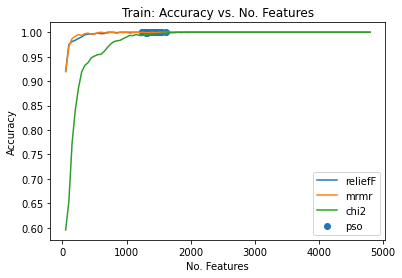
\includegraphics[width=\linewidth]{accuracy-features-fish-train.png}
    \caption{Species: Training set}\label{fig:fs-per-k-fish-train}
  \end{subfigure}
  \begin{subfigure}[b]{.55\linewidth}
    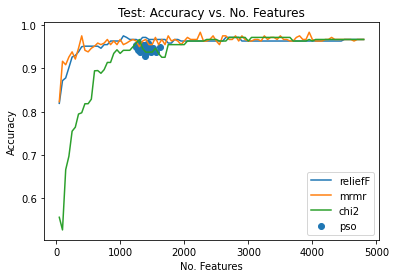
\includegraphics[width=\linewidth]{accuracy-features-fish-test.png}
    \caption{Species: Test set}\label{fig:fs-per-k-fish-test}
  \end{subfigure}
  \label{fig:fs-per-k-fish}
\end{figure}

Figure~\ref{fig:fs-per-k-fish} shows the results for Chi2, Relief-F, MRMR and PSO on the fish part species. 
We give the balanced classification accuracy for ten-fold cross-validation for each number of features selected $k$.
Where $k \in [0,50,...,4800]$, and $k$ increases by increment of 50.
In sum, this experiment gives 4 (feature selection methods) x 4800 (features) / (50) increment = 384 sets of empircal performance results. 

Figure~\ref{fig:fs-per-k-fish-train} (top) gives the training accuracy for fish species. 
All methods converge on optimal training accuracy at approximately $k = 1050$. 
The graph follows a plateau with $100\%$ accuracy, with diminishing returns past $k = 1000$. 
MRMR, Relief-F and PSO can fit the training data perfectly with approximately $k = 900$ features.
Chi2 is the slowest to converge, the algorithm performs poorly for low values of $k$. 
PSO achieves consistent train accuracy, it can perfectly fit the data dataset with $k$ features where $k \in [1100,1800]$. 

Figure~\ref{fig:fs-per-k-fish-test} (top) gives the test accuracy for fish species. 
The test graph has more variance than the training, with noise in accuracy for all methods. 
The graph stabilizes at a plateau with $96\%$ accuracy, with diminishing returns after $k=1100$. 
The test performance is worse than the training by $4\%$, suggesting some overfitting to the training set. 
The near-perfect $96\%$ test accuracy for fish species demonstrates the model can generalize well with (1100 selected / 4800 total) = 22.91\% features selected.
MRMR and Relief-F work best on the fish species dataset, they achieve the best test accuracy for $k \in [0,1200]$.
For MRMR and Relief-F, the model achieves 90\% test accuracy using only (50 selected / 4800 total) 1\% of its features.
PSO achieves its best test accuracies, with the smallest number of features selected. 
PSO performs worse on average than Relief-F and MRMR, although PSO found comparable results for its best individual runs. 

\subsection{Fish Part}

\begin{figure}[htb]
  \centering
  \caption[Two numerical solutions]{
      FS Classification Accuracy per $k$
    }
  \begin{subfigure}[b]{.55\linewidth}
    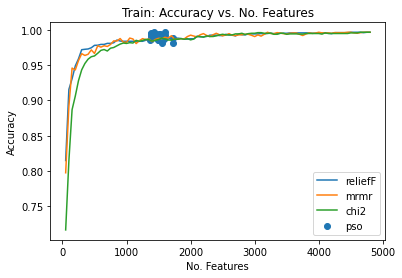
\includegraphics[width=\linewidth]{accuracy-features-part-train.png}
    \caption{Part: Training set}\label{fig:fs-per-k-part-part-train}
  \end{subfigure}
  \begin{subfigure}[b]{.55\linewidth}
    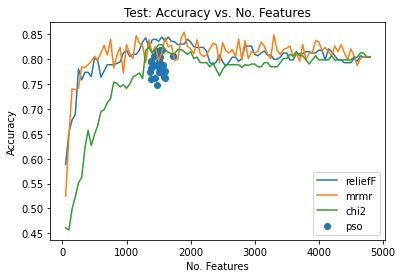
\includegraphics[width=\linewidth]{accuracy-features-part-test.png}
    \caption{Part: Test set}\label{fig:fs-per-k-part-part-test}
  \end{subfigure}
  \label{fig:fs-per-k-part}
\end{figure}

Figure~\ref{fig:fs-per-k-fish} shows the results for Chi2, Relief-F, MRMR and PSO on the fish part dataset. 
We give the balanced classification accuracy for ten-fold cross-validation for each number of features selected $k$.
Where $k \in [0,50,...,4800]$, and $k$ increases by increment of 50.
In sum, this experiment gives 4 (feature selection methods) x 4800 (features) / (50) increment = 384 sets of empircal performance results. 
 
% TODO [ ] - Rewrite all. 
% [x] - PSO achieves the best training accuracies with a much smaller number fo features. 
% [x] - Testing accuracy of PSO is not that good, potential overfitting, future work. 
% [x] - Other algorithms also achieve the best performance at around 1050 features, FS is helpful to improve the part classification. 
% [x] - Which algorithms work best on the species data. 
% [x] - Compare the performance of selected features and use all features.

Figure~\ref{fig:fs-per-k-part-part-train} (top) gives the training accuracy for fish part. 
For MRMR, Relief-F and Chi2 the train performance follows a log curve.
For these methods, there are sharp improvements between $k \in [0,1000]$, followed by a gradual incline, this peaks at the perfect fit on the training data when $k-4800$ (the entire feature set). 
PSO on average found smaller feature sets (low $k \in [1200,1600]$) with better train accuracy much faster than the other methods. 
PSO sometimes found solutions that fit the training data perfectly with $k = 1200$ features. 

Figure~\ref{fig:fs-per-k-part-part-test} (bottom) gives the test accuracy for fish part. 
PSO test accuracy is the worst, it performs worse than Relief-F, MRMR and Chi2. 
There is potential overfitting here, future work could address improving the generalization of PSO on test data. 
MRMR and Relief-F work best on the fish part dataset, they achieve the best test accuracy for $k \in [0,2000]$.
MRMR, Relief-F and Chi2 all achieve their best performance at $k = 1150$, notably better than using the whole feature set. 
For those methods, test accuracy decreases after $k = 1150$, a contrast to train accuracy which increases, this suggests the model overfits the training set when using too many features.
In comparison to fish species, the slope of the fish test contains far more variance, there is a lot of noise.
There is no clear signal, no smooth improvement in classification accuracy per k the graph shows the opposite. 
Feature selection improves the classification performance for the part dataset. 

\subsection{Disucssion}
\label{sec:results-feature-selection-discussion}

% Talking points: 
% Compare $\chi^2$ threshold to reliefF normalization term $m$, both parameters tuned by the algorithm. 

The MRMR and Relief-F methods performed the best for both datasets on the training data. 
A normalization term, $\frac{1}{|S|}$ for MRMR and $\frac{1}{M}$, are both used to scale the data, making them tolerant to noise. 
Chi2 performed the worst for species, this algorithm lacks a normalization term.
The $(.)^2$ operator makes this metric especially sensitive to outliers, outliers can often be attributed to noise. 
The use of normalization terms or lack thereof could explain why MRMR and Relief-F were robust in comparison to Chi2. 
The normalization term in the feature importance measure makes methods noise-tolerant. 

PSO performed worst for the fish part dataset.
Figure~\ref{fig:fs-per-k-part-part-test} shows a lot of noise, this would weaken the signal of the accuracy per k features. 
The accuracy per k features given in Figure~\ref{fig:fs-per-k-part-part-test}, can be seen as an approximation of the fitness function the PSO optimizes given in equation (\ref{eq:pso}).
The PSO noise in the part dataset increases the complexity of the fitness landscape where PSO searches for global optima. 
The accuracy per k features in figure~\ref{fig:fs-per-k-part-part-train} has less noise. 
For PSO, the fish part has a simpler fitness landscape than the fish species.
This explains why PSO can generalize to the test set better on fish species than the part. 

The PSO may not have a hyperparameter for feature number $k$.
Instead, it automates the selection of this parameter.
Yet, it achieves comparable results to other state-of-the-art methods.
This automation may prove useful for automating the classification task for online learning.
In a factory, we may want to train a model as new data arrives.
PSO requires less human intervention, yet still, for fish species provides competitive performance.

\section{Conclusions and Future Work}

% TODO [ ] Visualisation - I found no visualisation and interpretable models in this paper? 

This paper has demonstrated an interpretable and effective method for fish oil analysis. 
The method can be understood, domain experts can understand the important features in the decision-making.
Not only have we found effective classification and feature selection techniques, but we have also tried to explain their performance with visualisation and analytical results. 
We can draw many conclusions from the analytical results and visualisations, but here we recall the most important:

\begin{enumerate}
  \item Fish species are easier to predict than fish parts - there is more intra-class variation within fish species than there is a similarity between the same part from different fish.
  \item The Linear SVM classifier performs better for both classification tasks - the fish oil data is linearly separable on a hyperplane.
  \item Weight analysis of the SVM hyperplane serves as a useful approximation to gain insight into the model. This analysis is possible due to the nature of GC data, and its dot product with hyperplane coefficients of the Linear kernel. It is useful for troubleshooting/diagnosis using domain expertise. 
  \item This model can achieve 90\% fish species accuracy using only 1\% (k = 50) of its features, enabling efficient training, and showing many redundant and correlated features. 
  \item Feature selection improves the classification accuracy on the test set for the fish part - removing irrelevant features makes the task simpler. 
\end{enumerate}

LinearSVC applied to GC fish oil data can help to reduce waste in fish processing. 
Feature selection can be used to improve its performance, in terms of accuracy, efficiency and interpretability. 
Fewer features result in simpler models, which can be interpreted by domain experts to gain insight.
This ensures more sustainable eco-friendly practices in fish processing.
Waste reduction and repurposing is a rising tide that lifts all boats.
Sustainable practices will leave plenty of fish in the sea, preserving resources for future generations. 

% TODO [ ] - Future work: further steps, improve fish part performance, more challenging datasets, different tasks.

It is worth noting that the classification and feature selection methods presented in this paper could be extended to potentially improve performance. 
This is particularly useful for the lower-accuracy fish part dataset. 
Here we give a non-exhaustive list of possible extensions: 
(1) Further investigate feature selection by evaluating the FQC MRMR-variant proposed in \cite{zhao2019maximum}. 
% Zhao et al. \cite{zhao2019maximum} extend and evaluate existing MRMR variants, these consider different relevance and redundancy metrics.
% The FQC (F-test correlation quotient) MRMR variant proved robust and was put into production. 
(2) Extend classifier to S3VM \cite{zemmal2016adaptative}, a semi-supervised SVM that can utilize unlabelled GC data. 
This uses unlabelled data to ensure the decision boundaries are drawn through low-density areas.
(3) NIST has published a Gas Chromatographic Retention dataset \cite{kovats1958gas}. 
NIST could be applied to S3VM described, as well as pre-training/transfer learning approaches. 

% Please note that the first paragraph of a section or subsection is
% not indented. The first paragraph that follows a table, figure,
% equation etc. does not need an indent, either.

% Subsequent paragraphs, however, are indented.

% \subsubsection{Sample Heading (Third Level)} Only two levels of
% headings should be numbered. Lower level headings remain unnumbered;
% they are formatted as run-in headings.

% \paragraph{Sample Heading (Fourth Level)}
% The contribution should contain no more than four levels of
% headings. Table~\ref{tab1} gives a summary of all heading levels.

% \begin{table}
% \caption{Table captions should be placed above the
% tables.}\label{tab1}
% \begin{tabular}{|l|l|l|}
% \hline
% Heading level &  Example & Font size and style\\
% \hline
% Title (centered) &  {\Large\bfseries Lecture Notes} & 14 point, bold\\
% 1st-level heading &  {\large\bfseries 1 Introduction} & 12 point, bold\\
% 2nd-level heading & {\bfseries 2.1 Printing Area} & 10 point, bold\\
% 3rd-level heading & {\bfseries Run-in Heading in Bold.} Text follows & 10 point, bold\\
% 4th-level heading & {\itshape Lowest Level Heading.} Text follows & 10 point, italic\\
% \hline
% \end{tabular}
% \end{table}


% \noindent Displayed equations are centered and set on a separate
% line.
% \begin{equation}
% x + y = z
% \end{equation}
% Please try to avoid rasterized images for line-art diagrams and
% schemas. Whenever possible, use vector graphics instead (see
% Fig.~\ref{fig1}).

% \begin{figure}
% 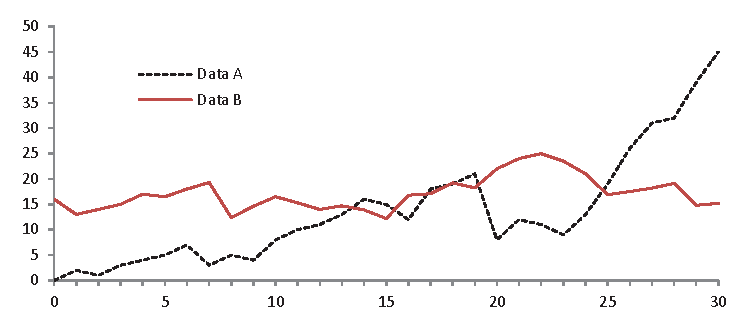
\includegraphics[width=\textwidth]{fig1.eps}
% \caption{A figure caption is always placed below the illustration.
% Please note that short captions are centered, while long ones are
% justified by the macro package automatically.} \label{fig1}
% \end{figure}

% \begin{theorem}
% This is a sampling theorem. The run-in heading is set in bold, while
% the following text appears in italics. Definitions, lemmas,
% propositions, and corollaries are styled the same way.
% \end{theorem}
%
% the environments 'definition', 'lemma', 'proposition', 'corollary',
% 'remark', and 'example' are defined in the LLNCS documentclass as well.
%
% \begin{proof}
% Proofs, examples, and remarks have the initial word in italics,
% while the following text appears in normal font.
% \end{proof}
% For citations of references, we prefer the use of square brackets
% and consecutive numbers. Citations using labels or the author/year
% convention are also acceptable. The following bibliography provides
% a sample reference list with entries for journal
% articles~\cite{ref_article1}, an LNCS chapter~\cite{ref_lncs1}, a
% book~\cite{ref_book1}, proceedings without editors~\cite{ref_proc1},
% and a homepage~\cite{ref_url1}. Multiple citations are grouped
% \cite{ref_article1,ref_lncs1,ref_book1},
% \cite{ref_article1,ref_book1,ref_proc1,ref_url1}.
%
% ---- Bibliography ----
%
% BibTeX users should specify bibliography style 'splncs04'.
% References will then be sorted and formatted in the correct style.
%
\bibliographystyle{splncs04}
% \bibliography{mybibliography}
\bibliography{refs}

\end{document}
